\chapter{Introduction}
\label{ch:chap1}


%------------------------------------------
\section{Backgrounds}

\subsection{Engineering Background}

Peripheral artery disease (PAD) is a major cause of amputation in United States. It is prevalent among smokers, diabetics and patient with dyslipidemia. Meanwhile, the long waiting time and high expense are two major problems for the patients. In the modern clinic room, the doctors are actively looking for a solution which can provide th both high fidelity and high resolution images to analyze the PAD. The  present technology can only render a two-dimensional,  monochrome, static and low-resolution picture. In recent decades, many researchers contribute numerous effort on improving the diagnosis of stenoses and the quality of images\cite{clark1976fluid, nesbitt2009shear, wardlaw2006non, stergiopulos1992computer, long2001numerical}. With the fast development on both hardware and computing algorithm, the computational simulations are aiming to provide 3D, dynamic, high resolution and patient-specific results. Comparing to current CT scan, it's significantly faster, cheaper and more accurate. In addition, it's also very important that the simulation results can bring the doctors and patients that the dynamic growth animations of current stenoses and the developing path after the clinic treatment. Fig \ref{fig: ch1f1} summarizes some factors which contributing to the interests in computational medical simulation technology\cite{barry2005features}. Many investigations have been conducted through last decades\cite{feng2012viscous, bertram2010evaluation, nadeem2010simulation, ogulu2005simulation}. However, since this is a fluid-structural interaction (FSI) problem, both high fidelity fluid and solid solvers are needed. 

\begin{figure}[H]
	\centering
	\begin{tabular}{c}
		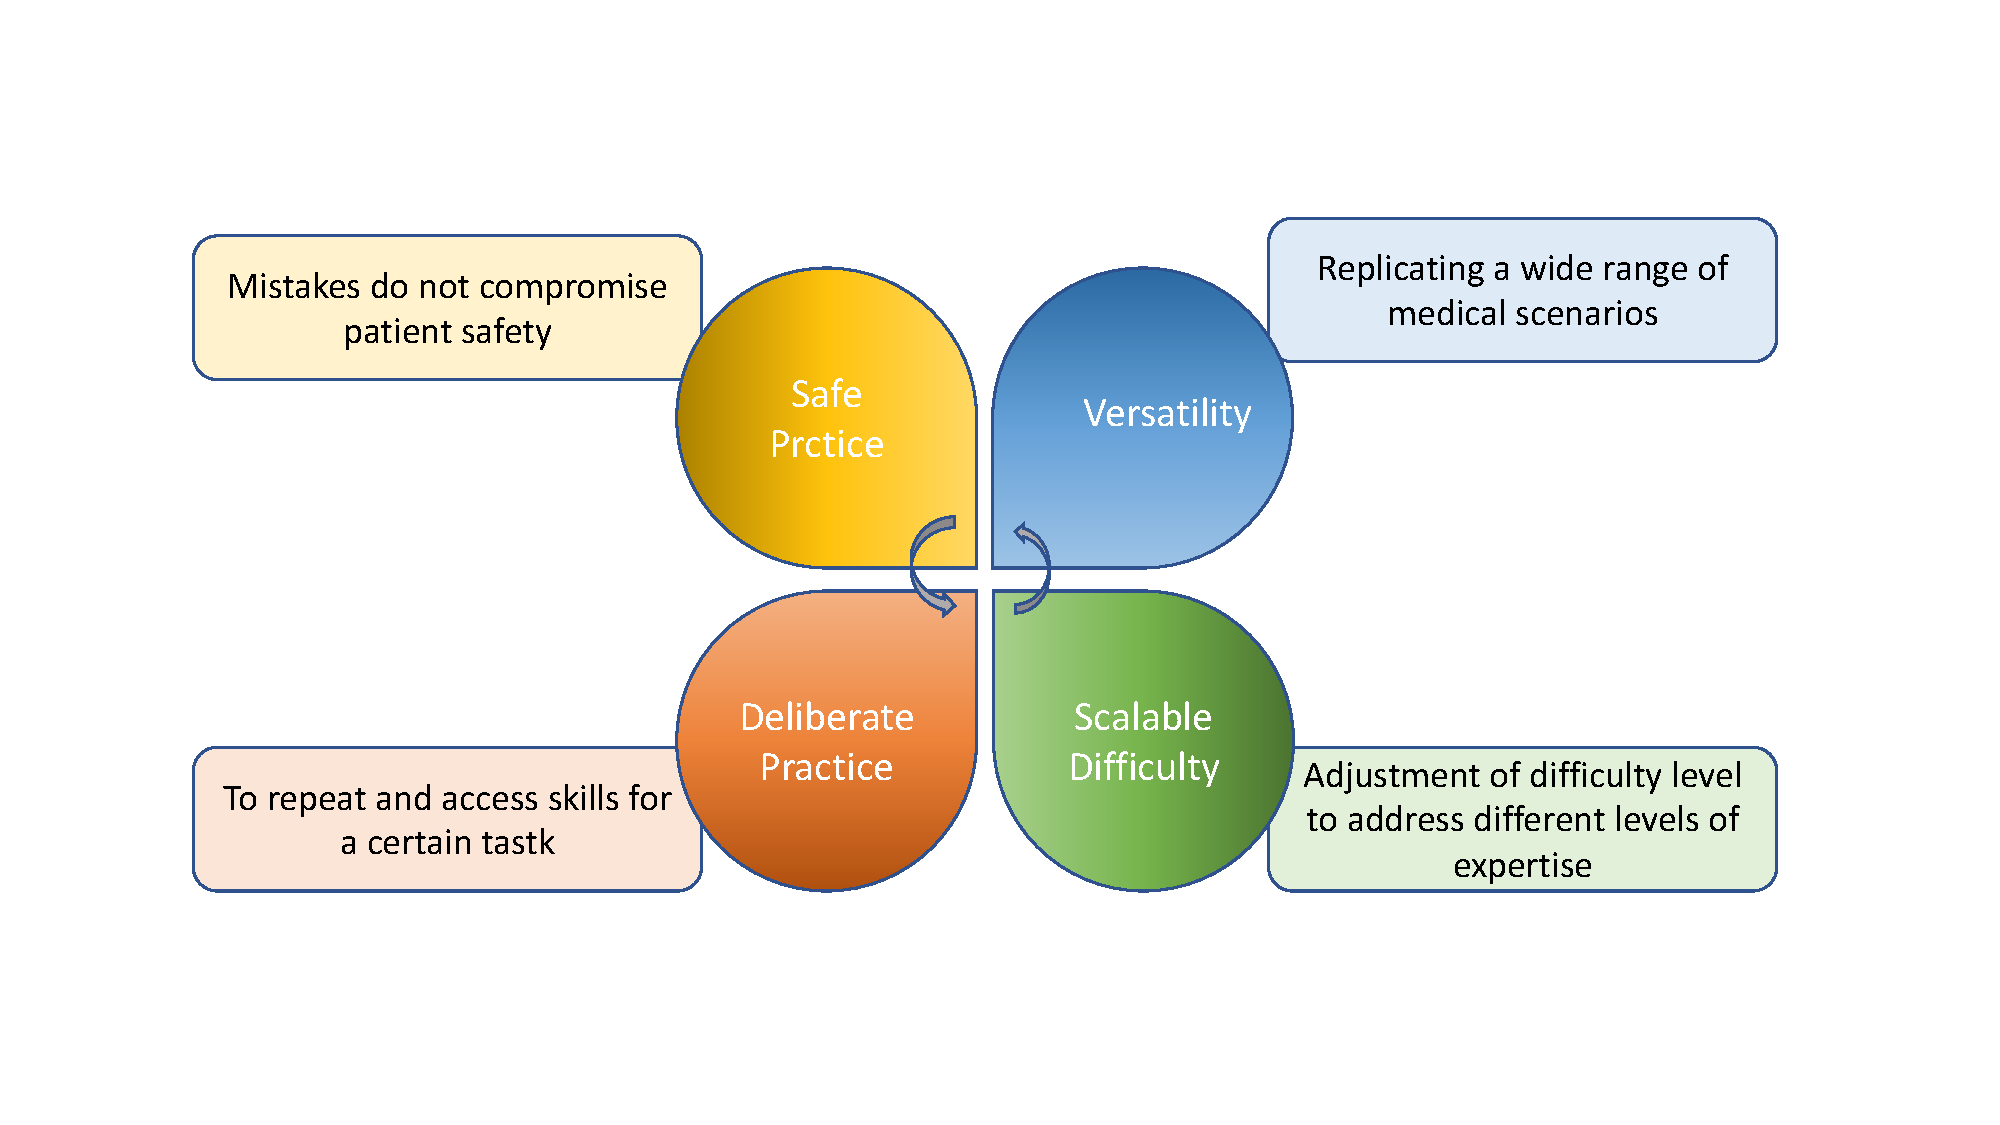
\includegraphics[width=1.0\textwidth]{./pics/computer_simulation}
	\end{tabular}
	\caption{\footnotesize Different factors affecting computer-based medical simulation.} \label{fig: ch1f1}
\end{figure}

Physically, the PAD can be abstracted as a fluid-structural interaction problem and be described by fluid and structure dynamics equations, respectively.  The two most popular approaches for solving such a FSI problem are monolithic method\cite{hubner2004monolithic, degroote2009performance} and partitioned method\cite{kuttler2008fixed, vierendeels2007implicit}. For the monolithic approach, the two sets of equations, fluid and structural, are solved simultaneously. The mutual influence on each other can be considered directly. One significant advantage of this scheme is its simplicity. Only a single global matrix is constructed so that both the fluid and structural parts can be solved under the same spatial discretization and time marching scheme. On the other hand, we lose the flexibility to separately control each partition. The other approach is partitioned method. The two sets of equations are solved separately and pass boundary conditions to each other like a cycle. The solution of fluid equations is calculated while the structural part waits for new input, and vice versa. A coupling algorithm to exchange the interaction solution between two phases as a pair of modules. The Implicit-Explicit (IMEX) Runge-Kutta (RK) time integration approach has been proved to be accurate and efficient on coupling the high order schemes\cite{zhang2016high}.

A Finite-Volume fluid solver \cite{liang2007large, liang2007large, liang2009effect} is accomplished and a series of CFD studies has been implemented on the idealized geometries. To implement a more high-fidelity simulation, the tissue of blood vessel wall shall be considered as elastic material. Therefore, an accurate and efficient solver for elasticity equation is needed. The solver should be capable of calculating the material behavior according to the stiffness property, which is the response of the deformable model reacting to the external forces. The simplest model is mass-spring model which is easy to compute but can not accurately determine the details of material behavior. A more precise approach is the finite element method, which is based on the continuum mechanics, has gained popularity. On the contrary to the mass-spring model, the FEM can specify the stiffness of the model by only using a few characteristic parameters, such as Young's modulus, Poisson ratio and the geometries. However, the challenge for 3D FEM simulation is its parallelization in large-scale parallel computational fluid-structure interaction frameworks is to be used in real-time application due to the very high computational expense. 

\begin{figure}[H]
	\centering
	\begin{tabular}{c}
		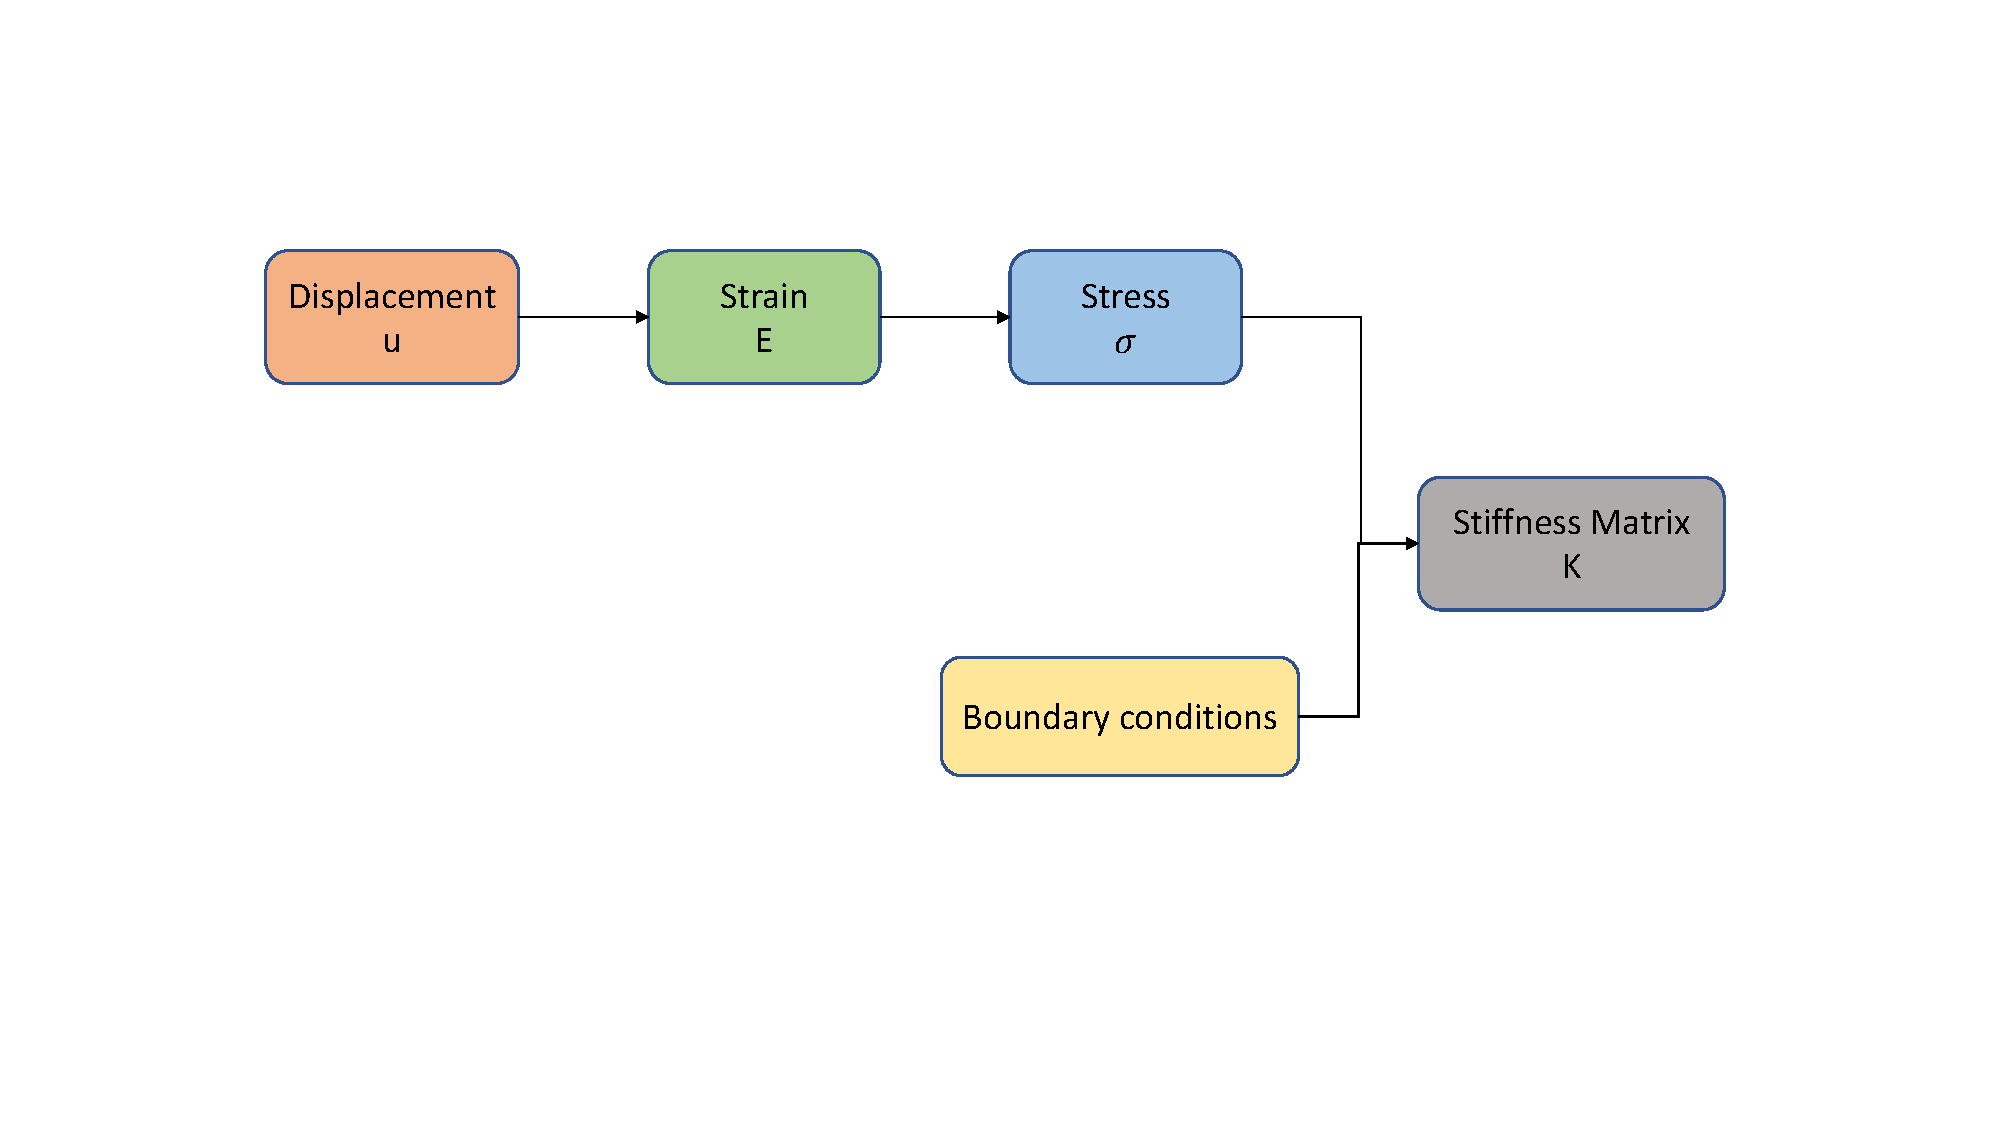
\includegraphics[width=1.2\textwidth]{./pics/construct_matrix}
	\end{tabular}
	\caption{\footnotesize Construct stiffness matrix.} \label{fig: ch1f2}
\end{figure}

Fig \ref{fig: ch1f2} shows a general process of calculating the stiffness matrix for a deformable material object. The stiffness matrix is derived from the gradient of stress which is calculated by the displacement and material property. The boundary conditions are imposed upon the contact interaction.

\begin{figure}[H]
	\centering
	\begin{tabular}{c}
		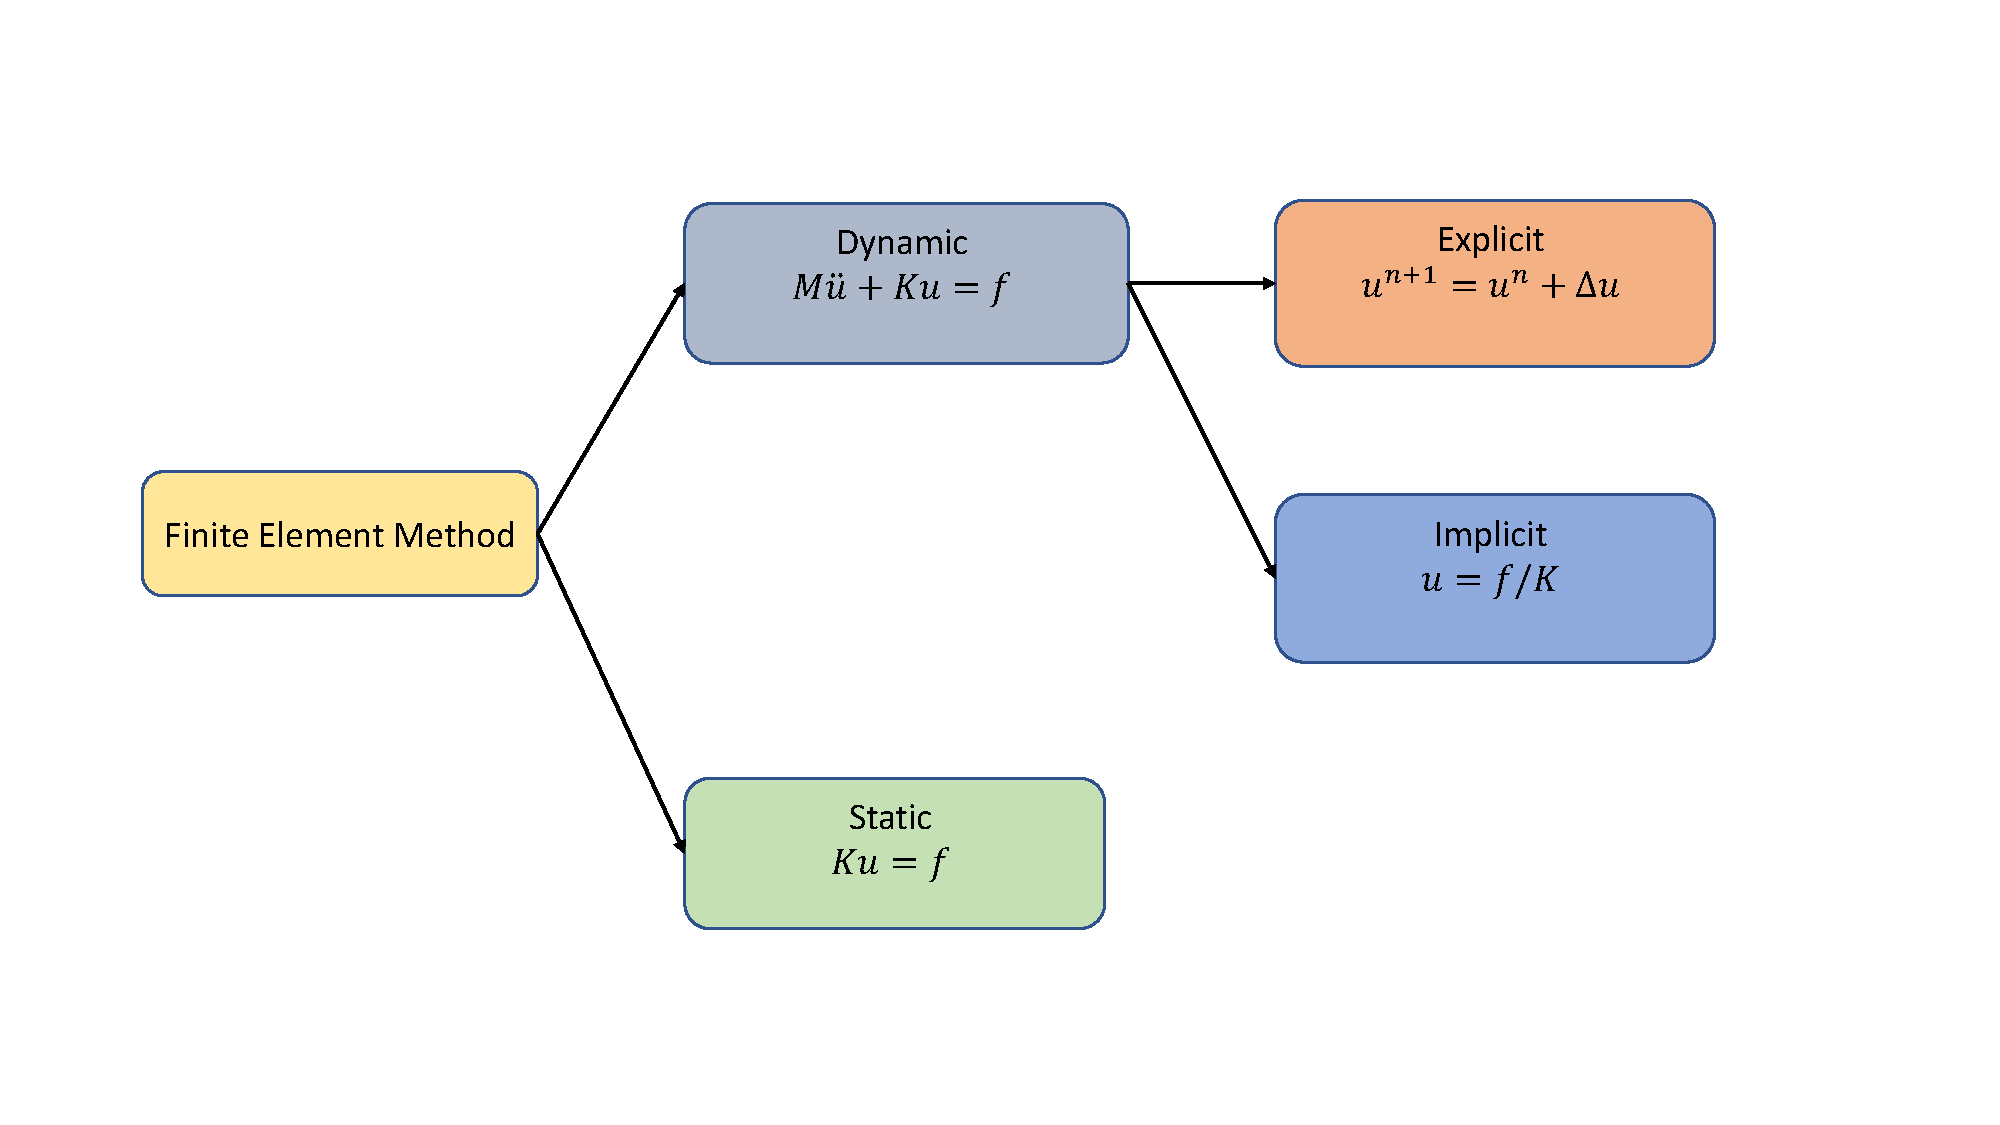
\includegraphics[width=1.1\textwidth]{./pics/fem}
	\end{tabular}
	\caption{\footnotesize Static and dynamic finite element method.} \label{fig: ch1f3}
\end{figure}

The Fig \ref{fig: ch1f3} displays both static analysis and dynamic analysis for a set of linear system of elasticity equations. The steady-state and transient finite element problem are studied with static analysis and dynamic analysis respectively. The latter is time dependent. In dynamic analysis, we shall consider the spatial discretization by using both explicit and implicit time integration schemes\cite{bathe2008finite}. The implicit time marching scheme is computationally costly, because the matrix inversion for large linear system is required every time-step, similar to solving the static problem. The benefit is unconditionally stable for large time step. On the other hand, the explicit time marching scheme requires much less computational cost as no linear solver is involved for each time-step. However, the size of each time step has to satisfy the numerical stability criteria. 


Commonly, the linear system of elasticity equations derived from the FEM method is positive definite and too large to be direct inverse. The most time consuming part in the FEM analysis in Fig \ref{fig: ch1f2} is solving the linear system. The complex system can be written in a matrix form $ \mathbf{A} \mathbf{x} = \mathbf{b} $. To solve it, there are two main categories of algorithms, directive method and iterative method. Considering the better performance on memory usage and computing time, the iterative method gains more affirmatives\cite{brussino1989comparison} for large scale problems. The Preconditioned Conjugate Gradient (PCG) is the one of the most popular method because of its robustness and fast convergence. However, the PCG requires positive definite matrices. It is still very challenging to implement finite element analysis using implicit scheme to study the material real-time response behavior because of excessive computational cost. Therefore, the domain decomposition method combined with parallel computing scheme is one emerging choice to reduce computational cost.

Parallel computing desires great load balancing in order to achieve competitive concurrent execution in terms of computational time. The challenges to reach that purpose includes learning and understanding programming paradigms,  balance the loads to maximize the usage of bandwidth, minimize the overhead on data communication and avoid potential data racing problems. To achieve good level of parallelism, we employ some modern techniques such as MPI, Intel Math-Kernel library and LAPACK-BLAS for optimal scalability by reducing the overhead latency with a large number of active processors and ensure the balance of loads on each processor.

\subsection{Overview of Related Numerical Methods}

The Weak Galerkin Finite Element Method (WG-FEM)is a novel developed, effective numerical method for solving partial differential equations. The WG method is first proposed by Dr. Junping Wang and Xiu Ye in 2011, then applied for solving second order elliptic equations\cite{wang2014weak}. The WG method introduces a series of weak operators such as weak gradient, weak divergence and weak curl operators for the computation of corresponding strong forms of differential equations. The WG finite element method provides a  new perspective to solve numerical problems. The WG method can be applied on variety of partial differential equations include second order elliptical equation, elasticity equation\cite{wang2016locking}, Stokes equations \cite{wang2016weak} and Maxwell's equations \cite{mu2013weak}, etc. The WG method inherits the discontinuity from the continuous basis functions per element. The construction of discrete matrices are independent with of external coefficients. The interior unknown variables can be projected to the boundary unknown variables to construct a linear system which only consists of degrees of freedom(DOFs) along the element boundary. In short, even though the total DOFs of WG method is larger than the Discontinuous Galerkin method (DG), the interior unknown variables can be eliminated through Schur complement method. The only remaining DOFs are along the element boundary which are far less DOFs than those in DG finite element method. The elemental stiffness matrix of WG method can be constructed for each element, which is consistent with CG FEM method. 

%-----------------------------------------------------
\section{Objective}

The CG FEM analysis of continuum mechanics is widely used to study and predict material deformations. The results are generally accurate and reliable for analyzing the relationship between load and deformation. However, the computational complexity and cost prevents its the application to large-scale FSI problems. Massive parallel computing is required for obtaining large linear system. In this work, we investigate the methods for efficient parallel scheme which enables high-order novel finite element method for solving large scale elasticity equation.

We employ the WG-FEM to convert the bilinear form equations into a positive definite linear system. The WG method can use various types of different elements. The selection of polynomials on interior or boundary region is flexible which enhances the freedom of computational simulation for dealing with complex geometries. Moreover, the discontinuous features in the WG method which empowers the parallel computation capability.

The Balancing Domain Decomposition by Constraints (BDDC) method is an ideal candidate for enabling the massive parallel capacity to WG-FEM. BDDC identifies the two spaces (primal and dual) and apply the divide and conquer strategy to the original computational domain. By minimizing the global communication and synchronization overhead,  WG-BDDC empowers the scalability of elasticity equations as a superlinear speedup curve.

The main objective of this dissertation is to deliver high speed, accuracy and scalability in WG-BDDC based analysis. Fig \ref{fig: ch1p4} shows the paths to accomplish the objectives in this work. The results of the research significantly improves the computation of the elastic material response, including in clinic judgment and other medical applications.

\begin{figure}[H]
	\centering
	\begin{tabular}{c}
		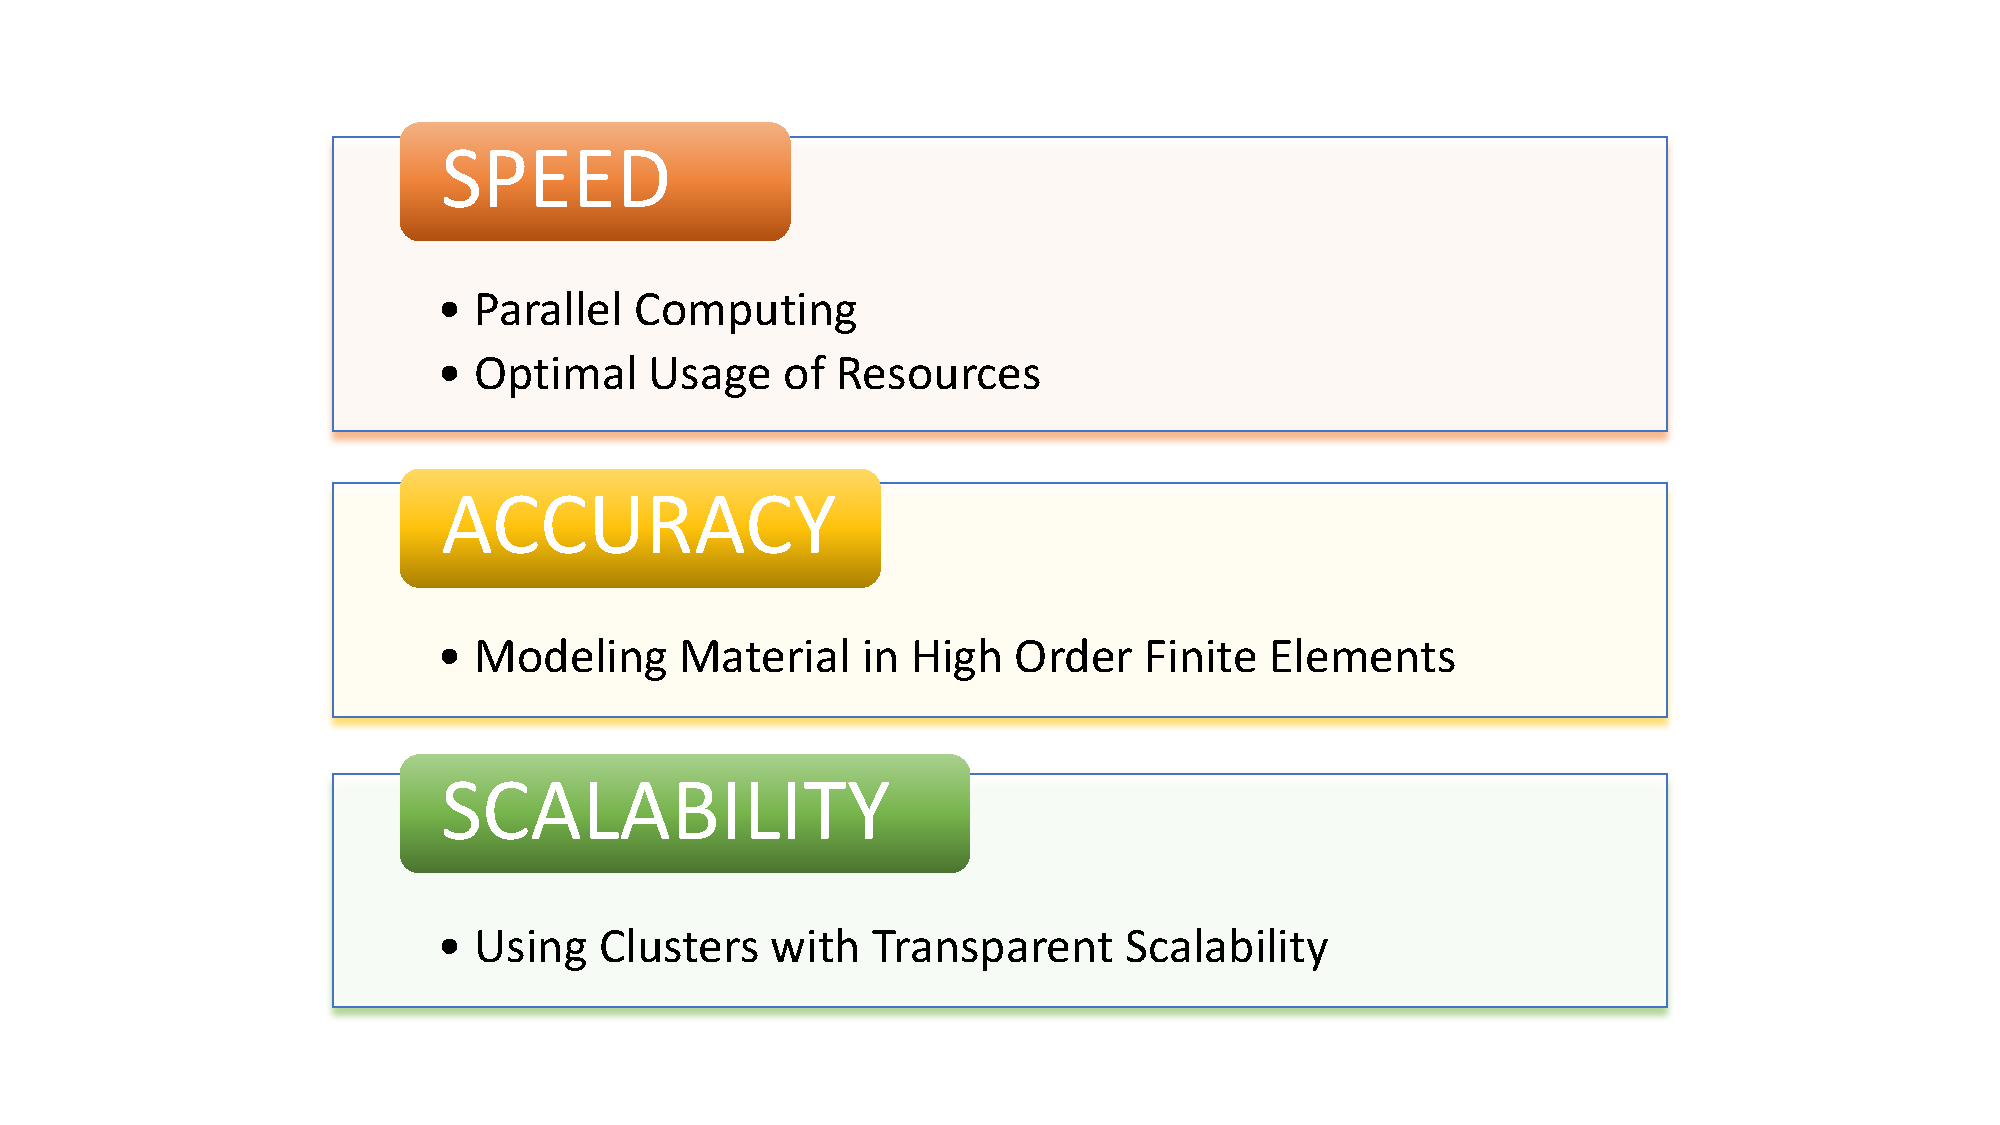
\includegraphics[width=1.0\textwidth]{./pics/ch1p4}
	\end{tabular}
	\caption{\footnotesize Objectives and methodology.} \label{fig: ch1p4}
\end{figure}

To validate the WG-BDDC scheme and develop the software, we first design the hybrid WG-CG element. The results are consistent with the benchmark of CG only element so the fidelity is proved. Then we extend the WG element to BDDC method and verify the properties of convergence and the order of accuracy with parallel fashion. Finally, the scalability is discussed under the parallel computing framework.

The rest of this dissertation is organized as :

\begin{itemize}
	\item Chapter 2 presents the background and basics of WG method.
	\item Chapter 3 discusses the hybrid WG-CG element the performance on nonlinear elasticity equation.
	\item Chapter 4 introduces the WG-BDDC method for second order elliptic and elasticity equation.
	\item Chapter 5 shows the study of effect multiple stenoses on the peripheral artery diseases.
	\item Chapter 6 concludes this work and outlook the future work.
\end{itemize}
